\documentclass[12pt]{article}
\usepackage{graphicx}

\usepackage[margin=1in]{geometry}
\usepackage{float}
\usepackage{listings}

\title{Labwork 4: Threads}
\author{Ngo Quang Truong 2540106}
\date{1 Oct 2026}

\begin{document}

\maketitle
\newpage

\section{Introduction}

This report presents an implementation of RGB image-to-grayscale conversion using both a traditional 2D CPU approach and a 2D CUDA-based GPU approach.

\section{Method}
An RGB image represents each pixel using three color components: red ($R$), green ($G$), and blue ($B$). The grayscale value is calculated using the weighted sum: 
\begin{equation}
g(y,x) = \frac{1}{3}\sum_{i=0}^{2} I(y,x,i)
\end{equation}

\section{CPU Implementation} 
The CPU implementation processes the image sequentially, converting each RGB pixel to grayscale while preserving the original 2D image structure rather than flattening it into a 1D array. For the test image, the 2D implementation takes 9.15 seconds, compared with 7.028 seconds for the 1D implementation, making the 2D approach approximately slower than the flattened 1D approach.

\begin{figure}[h]
    \centering
    
\includegraphics[width=0.5\textwidth]{original_image.jpg}
    \caption{Original RGB image}
    \label{fig:original_image}
\end{figure}

\begin{figure}[H]
    \centering
    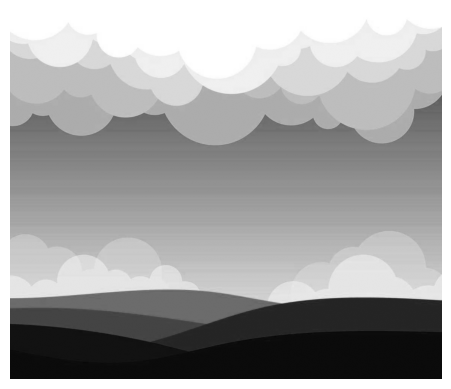
\includegraphics[width=0.5\textwidth]{cpu_output.png}
    \caption{CPU Grayscale image}
    \label{fig:cpu_processed}
\end{figure}

\section{CUDA GPU Implementation}

The second implementation uses CUDA through the Numba library to accelerate the grayscale conversion on the GPU. Unlike the previous lab, where the image was flattened into a 1D array, this implementation preserves the original 2D image structure.  For the same test image, the CUDA implementation in 2D slightly slower than 1D, 0.129665 seconds comared to 0.094863 seconds.
\begin{figure}[H]
    \centering
    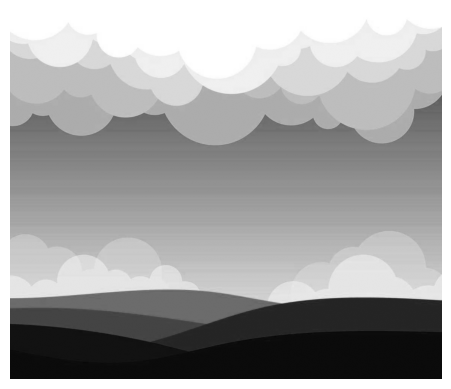
\includegraphics[width=0.5\textwidth]{gpu_output.png}
    \caption{GPU Grayscale image}
    \label{fig:GPU_processed}
\end{figure}


\end{document}